% ----------------------------------------------------------
% Implementação
% ----------------------------------------------------------
\chapter[Implementação]{Implementação}\label{chap:implementacao}

\section{Tecnologias e ferramentas}

\subsection{JavaScript}

No início da Internet, os únicos documentos transferidos eram páginas estáticas HTML. Nenhuma página possuía conteúdo dinâmico e nem possibilidade de interação com a mesma. Javascript foi idealizado com esse intuito. Desenvolver uma forma com que os usuários possam realizar ações e receber resultado de forma mais rápida. A web precisava ser mais dinâmica, de acordo com Marc Andressen, fundador da Netscape Communications\footnote{Disponível em: <https://auth0.com/blog/a-brief-history-of-javascript/>. Acesso em 20 mai. 2018.}.

Criada em 1995, no meio da chamada \textit{browsers war} (ou guerra dos navegadores). Foi desenvolvida em apenas dez dias por Brendan Eich, e a princípio levou o nome \textit{Mocha}. Em agosto do mesmo ano, a Netscape em parceria com a Sun Microsystems (criadora da linguagem Java, posteriormente adquirida pela Oracle) apresentou o  Javascript\footnote{Disponível em: <http://tech-insider.org/java/research/1995/1204.html>. Acesso em 20 mai. 2018.}, com o intuito de torná-la a linguagem de script oficial dos navegadores.

Javascript na verdade é uma implementação/extensão da especificação ECMAScript (\cite{ecmascript}), desenhada para facilitar a padronização de  linguagens proprietárias baseadas na ECMAScript, como por exemplo JScript, a linguagem de script da Microsoft. Essa especificação define uma linguagem com paradigma orientado a objetos, tipagem fraca e que funciona através de interpretadores, ou seja, não compilada (diferentemente de Java, apesar do nome).

A grande diferença entre a especificação e a implementação são as interfaces de aplicação disponíveis na linguagem executada pelos navegadores. Como por exemplo, a API voltada para interação com HTML, chamada de DOM ou \textit{Document Object Model}, que foi a primeira responsável pelo maior dinamismo das páginas da Internet. Hoje em dia temos interfaces para captura de mídia (áudio, vídeo); interação com dispositivos móveis (bateria, GPS); e até para conexões \textit{peer-to-peer}, assunto do presente trabalho.

Cada vez mais utilizada devido a sua presença na Web, muitos desenvolvedores acreditaram que a linguagem era digna de funcionar também no servidor, eliminando a necessidade de navegadores. Com o lançamento da \textit{engine} V8, o interpretador desenvolvido pela Google para ser utilizado no seu navegador Chrome, a linguagem atingiu um outro nível de utilização, passando a ser utilizada também em servidores, através do ambiente Node.js. Denominado \textit{cross platform}, o Node.js é capaz de ser executado em qualquer sistema operacional e funciona em cima do interpretador V8, tornando a linguagem livre das amarras dos navegadores. A linguagem também pode ser encontrada em aplicações de banco de dados não-relacionais, como o MongoDB.

Nesse projeto, Javascript será utilizado tanto no cliente como no servidor (com exceção do banco de dados). Devido a isso, o primeiro item do tópico de tecnologias foi uma introdução à mesma. Abordaremos nos próximos itens como esta linguagem será utilizada no projeto.

\subsection{Servidor}
%FRANK: Essa subseção ficou confusa. Mistura a tua proposta com tecnologias utilizadas. Sugiro separar bem essas duas coisas.
%LUCAS: Movi a subseção de projeto para implementação

Servidor constituído de uma API e uma conexão com WebSockets. A interface REST servirá para enviar e receber dados de sobre os atendimentos do banco de dados. Utilizaremos WebSockets para realizar as conexões P2P nas videoconferências.

Composto por \textit{frameworks} e bibliotecas desenvolvidos com a plataforma NodeJS. Utiliza o gerenciador de pacotes NPM ou \textit{Node Package Manager} para instalação das dependências do projeto.

ExpressJS é a ferramenta utilizada para criação da API REST que servirá para enviar e receber dados sobre os atendimentos do banco de dados. Responsável também por devolver uma página HTML a ser integrada no cliente.

SocketIO fornece uma interface de aplicação em cima de uma conexão por WebSockets e auxiliará as conexões \textit{peer-to-peer}.

E por final possui uma biblioteca, chamada ObjectionJS. Funciona como um ORM ou \textit{Object Relational Mapping}, tornando mais fáceis as operações no banco de dados.

\subsubsection{ExpressJS}

Um dos primeiros e mais famosos \textit{frameworks} desenvolvidos para servir aplicações Web com NodeJS. Tornou-se popular pela sua facilidade de uso, alta possibilidade de customização e suporte a ferramentas de linha de comando. Observamos em seu site\footnote{Disponível em: <http://expressjs.com/>. Acesso em 15 mai. 2018.} o foco em se manter como uma ferramenta minimalista e \textit{unopinionated}, que tem como objetivo dar mais controle aos desenvolvedores, diferentemente de grandes \textit{frameworks} como Ruby On Rails.

Possui uma arquitetura voltada a \textit{middlewares}\footnote{Disponível em: <https://www.cleveroad.com/blog/the-best-node-js-framework-for-your-project--express-js--koa-js-or-sails-js>. Acesso em 20 mai. 2018.}. Esse tipo de arquitetura suporta o registro de módulos que são executados em ordem a cada ciclo de requisição e resposta HTTP. Devido a sua  natureza minimalista, a maior parte das customizações do servidor são feitas através dos \textit{middlewares}. Esses são responsáveis por adições de cabeçalhos HTTP, abertura de conexão com o banco de dados, autenticação de usuário, dentre outras.

Todas as funcionalidades presentes no ExpressJS poderiam ser implementadas com NodeJS puro. De acordo com \ref{lst:express_server}, o \textit{framework} traz aos usuários ferramentas para desenvolver servidores HTTP com rapidez e simplicidade, permitindo implementar um servidor com apenas algumas linhas de código:

\begin{lstlisting}[caption={Servidor ExpressJS}, label={lst:express_server}]]
var express = require('express');
var app = express();
app.get('/', function(req, res) {w
	res.send('<h1>Hello World!</h1>');
});
app.listen(8000);
\end{lstlisting}

Toda essa simplicidade e liberdade de customização vem com certos custos. A aplicação de um time pode acabar muito diferente de outros, o que não acontece em \textit{frameworks} com padrões bastante definidos, como por exemplo Django, escrito em Python.

Devido a sua rapidez, utilizaremos ExpressJS para construir uma API RESTful, responsável por salvar e trazer os dados dos usuários conectando com o banco de dados através de uma biblioteca.

\subsubsection{SocketIO}

SocketIO é um \textit{framework} escrito em Javascript voltado para aplicações web em tempo real.

A arquitetura é baseada em um sistema com padrão baseado em eventos e funciona de forma bi-direcional, ou seja, do navegador ao servidor e vice-versa. É constituída de um servidor implementado com Node.js e uma biblioteca Javascript que realiza a conexão a partir do cliente.

Para efetuar a comunicação em tempo real os contribuidores do projeto desenvolveram o protocolo SocketIO\footnote{Disponível em: <https://github.com/socketio/socket.io-protocol>. Acesso em 24 mai. 2018.} que foi em seguida implementado pelo \textit{framework}. O documento descreve uma arquitetura que realiza o \textit{Upgrade} de uma conexão HTTP para WebSockets se suportado e caso não seja usa como \textit{fallback} outras alternativas, como \textit{long-polling}.

Apesar de utilizar conexões WebSockets (quando possível), o \textit{framework} não é uma implementação da especificação. Age como uma interface de aplicação encapsulando uma \textit{engine}/biblioteca  que funciona de acordo com o protocolo WebSocket, como podemos ver no relatório de mudanças da versão 2.0\footnote{Disponível em: <https://socket.io/blog/socket-io-2-0-0/>. Acesso em 24 mai. 2018.}.

Ao invés de usarmos somente uma biblioteca que implemente o protocolo WebSockets ou logo a interface nativa do navegador, optamos por essa ferramenta mais robusta devido a algumas funcionalidades descritas na página de documentação\footnote{Disponível em: <https://github.com/socketio/socket.io/\#features>. Acesso em 24 mai. 2018.}:

\begin{itemize}
	\item Suporte a \textit{multiplexing}: facilita a comunicação em diferentes canais, porém utilizando a mesma conexão;
	\item Confiabilidade: consegue conectar-se mesmo através de \textit{proxies} e \textit{firewalls}; e
	\item Suporte reconexão automática em caso de perda de conexão.
\end{itemize}

Observamos na listagem \ref{lst:socketio_server} como é simples a integração com um servidor NodeJS. Iniciamos o servidor executando a função \textit{createServer} onde registramos uma aplicação ExpressJS. Na quarta linha é criado um objeto \textit{io} que atua como um barramento de eventos, escutando por eventos \textit{connection} que no projeto utilizaremos para realizar as conexões P2P.
%FRANK: explique em poucas palavras o que o código da figura faz. 
%LUCAS: Alterado em 01/06

\begin{lstlisting}[caption={Servidor ExpressJS integrado com SocketIO}, label={lst:socketio_server}]
var express = require('express');
var app = express();
var server = require('http').createServer(app);
var io = require('socket.io')(server);
io.on('connection', function(){ /* */ });
server.listen(3000);
\end{lstlisting}

O projeto integrará o framework no servidor para troca de informações sobre \textit{peers} de uma videoconferência para que então os navegadores possam realizar a conexão P2P entre eles e eliminar a necessidade do servidor.

\subsubsection{ObjectionJS}

ORM ou \textit{Object Relational Mapping} é uma técnica relacionada a manipulação e conversão de dados. Consiste em mapear elementos de um banco de dados, como tabelas, colunas e linhas para o paradigma orientado a objetos. 

Geralmente quando nos referimos a ORM, estamos dizendo uma biblioteca que implementa essa técnica,encapsulando o código responsável por fazer \textit{queries}, inserções e atualizações no banco, e abstraindo o programador de linguagens como SQL e NoSQL.

Para esse projeto foi escolhido uma biblioteca chamada ObjectionJS\footnote{Disponível em: <https://vincit.github.io/objection.js/\#introduction>. Acesso em 29 mai. 2018.}, desenvolvida para servidores NodeJS e que integra-se facilmente com \textit{framework} ExpressJS. Com essa ferramenta conseguimos agilizar o processo de desenvolvimento através de mapeamentos das entidades do banco de dados (como no exemplo da Listagem \ref{lst:user_model_mapping}) para modelos no servidor, evitando a utilização de códigos  SQL e aproveitando técnicas com \textit{lazy loading} fornecida pela biblioteca.

\begin{lstlisting}[caption={Mapeamento modelo User}, label={lst:user_model_mapping}]
const { Model } = require('objection');
	
export class User extends Model {
	static tableName = 'users';
	static idColumn = 'id';
	  
	fullName() {
		return this.name + ' ' + this.lastName;
    }
}
\end{lstlisting}

ObjectionJS tem suporte testado e garantido para três gerenciadores de banco de dados, que são SQLite3, PostgreSQL e MySQL. Devido à sua grande popularidade, utilizaremos o segundo da lista, PostgreSQL.

\subsection{Cliente}

Os navegadores atuais suportam as seguintes tecnologias para renderização de páginas: HTML, CSS e Javascript. Com a popularidade da Web, surgiram comunidades e empresas interessadas pelo avanço da Internet. Em conjunto, esses dois grupos designaram órgãos responsáveis por manterem especificações e padrões de cada uma dessas tecnologias, por exemplo a W3C ou \textit{World Wide Web Consortium}.

Devido à grande diversidade de \textit{browsers} existentes e cada um deles apostando em sua própria implementação, o avanço dos navegadores ficou estagnado e anda relativamente devagar em comparação a outras ferramentas de desenvolvimento.

Com essa demora para atualização dos \textit{standards}, desenvolvedores decidiram agilizar o processo e utilizar recursos que ainda não foram padronizados. Existem diversas bibliotecas, ferramentas de linha de comando e empacotadores de módulos que \textit{transpilam\footnote{Compilar de uma linguagem para outra, porém no mesmo nível de abstração}} uma versão mais nova do Javascript para o suportado oficialmente pelos navegadores.

A parte que compreende o cliente na nossa arquitetura envolve tecnologias que auxiliam esse avanço.

\subsubsection{Webpack}

Navegadores atualmente não suportam oficialmente o conceito de módulos Javascript. Existem duas opções para melhor organizar o código em grandes projetos: dividir o código em vários arquivos de script e utilizar mais de uma chamada no servidor para executá-los na página; ou agrupar todo o código em um só arquivo e realizar somente uma requisição HTTP.

A segunda opção é a mais difundida em projetos com uma estrutura complexa. No navegador, para que a separação de módulos seja bem sucedida a ordem de importação dos scripts deve ser respeitada e dependendo da quantidade a importação pode impactar bastante na performance da aplicação, devido à abertura de diversas conexões HTTP. Reunir todos os módulos necessários e importá-los na ordem correta manualmente não é viável para times ágeis que prezam pela produtividade e a escalabilidade de um produto.
%FRANK: reveja o final do último parágrafo, sobre a queda de performance...
%LUCAS: Alterado 01/06

Para atingir esse objetivo, será utilizado o empacotador de módulos Webpack\footnote{Disponível em: <https://webpack.js.org/>. Acesso em 29 mai. 2018.}. Em sua configuração mais simples, necessita de um arquivo de configuração na raiz do projeto que indique um ponto (arquivo) de entrada e a pasta de saída, onde será armazenado o resultado do empacotamento. Esse resultado, normalmente referido como \textit{build}, é constituído de arquivos CSS, Javascript e uma página HTML responsável por importar e executar os scripts.

\subsubsection{ReactJS}

Javascript é por design uma linguagem orientada a objetos e imperativa. Com o aumento da popularidade de linguagens funcionais na comunidade, surgiram diversas bibliotecas que trazem técnicas funcionais para o Javascript, incluindo React.

O React é uma biblioteca Javascript desenvolvida pelo Facebook voltada para construção de interfaces, ou seja, compreende o V em um arquitetura MVC (\textit{Model-View-Controller}).

React introduziu uma forma de escrever interfaces quando apresentou uma nova linguagem de script que transpila para Javascript puro, chamada JSX. JSX possibilita o uso de uma sintaxe similar à linguagem de marcação HTML (declarativa por design) dentro de scripts JS. 
%FRANK: explicar melhor a listagem
%LUCAS: arrumei e alterei a explicação para baixo do código 01/06

\begin{lstlisting}[caption={Exemplo de componente escrito com JSX}, label={lst:react_jsx}]
function formatName(firstName, lastName) {
  return firstName + ' ' + lastName;
}

function Component({ firstName, lastName }) = {
  return (
  	<h1>
		Hello, {formatName(firstName, lastName)}!
  	</h1>
  );
}

render(
	<Component firstName="John" lastName="Doe" />
);
\end{lstlisting}

No código \ref{lst:react_jsx} observamos o uso tanto de \textit{tags} HTML, quanto de funções imperativas. A função \textit{formatName} é padrão da linguagem Javascript, porém a \textit{Component} define um dos conceitos mais importantes da biblioteca React, o componente.

Outra característica semelhante a linguagens funcionais é a ideia de funções puras\footnote{Disponível em: <https://medium.com/javascript-scene/master-the-javascript-interview-what-is-a-pure-function-d1c076bec976>. Acesso em 29 mai. 2018.}. Uma função normal pode ser pura se: para o mesmo argumento de entrada sempre retornar o mesmo resultado; e não produzir efeitos colaterais, ou seja, alterar algum dado fora do seu escopo interno. Esse tipo de função é popular devido a sua previsibilidade, clareza e facilidade de testar.

A biblioteca tem uma arquitetura baseada no desenvolvimento orientado a componentes, o que significa que as interfaces resultantes de projetos React são construídas a partir de composições dos mesmos. Esses componentes são as funções puras da biblioteca e idealmente devem ser encapsulados, com objetivo definido e retornar o mesmo resultado sempre que os atributos\footnote{\textit{firstName} e \textit{lastName} em \ref{lst:react_jsx}} declarados sejam iguais.
%FRANK: rever a última frase do parágrafo (Encapsulados...)
%LUCAS: corrigido 01/06

Escolhida para o desenvolvimento da interface devido a sua popularidade na comunidade, pela sua facilidade de uso, apesar de um alta curva de aprendizado e o aspecto funcional e declarativo.

\section{Desenvolvimento do sistema}

Com base na modelagem de classes e nos casos de uso levantados foi criado uma arquitetura para suprir as necessidades do sistema e do problema apresentado no trabalho.
O projeto foi desenvolvido utilizando Git para controle de versão junto do sistema Github para subir o código em um repositório online. 

\begin{figure}[ht!]
	\centering
    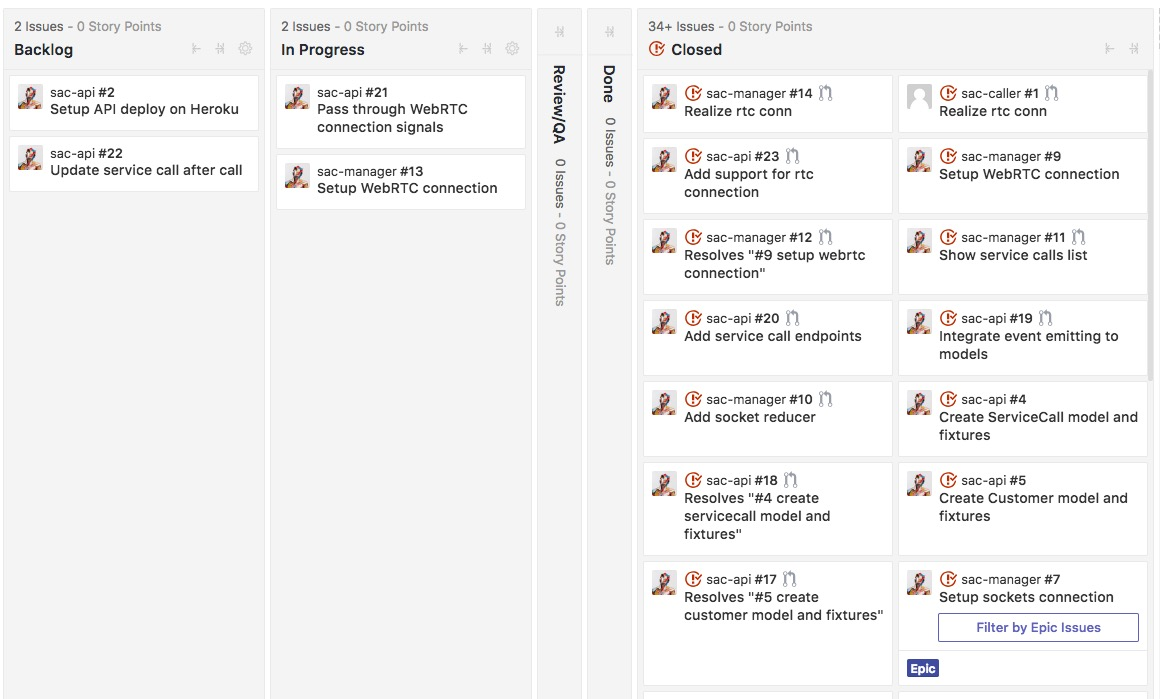
\includegraphics[scale=0.35]{figures/zenhub-tickets.jpg} 
	\caption{Organização do projeto dentro do Github/ZenHub}
	\label{fig:zenhub_tickets}
\end{figure}

Foi utilizada a extensão ZenHub (\autoref{fig:zenhub_tickets}) para organização e gerenciamento de tickets com uma metodologia similar ao Kanban. O sistema é constituido de quatro projetos, \textit{SAC API}, \textit{SAC Manager}, \textit{SAC Caller} e \textit{SAC Plugin}e abaixo será explicado sua arquitetura.

\clearpage
\subsection{Arquitetura}

Pensada de maneira a fornecer ao usuário do sistema de atendimento uma facilidade ao se conectar com seu próprio cliente. A decisão em dividir o projeto em múltiplas partes veio da necessidade do \textit{sac-caller} ser usado em dispositivos móveis, ou seja, era necessário uma aplicação pequena que não consumisse muita internet ao baixá-la.

\begin{figure}[ht!]
	\centering
    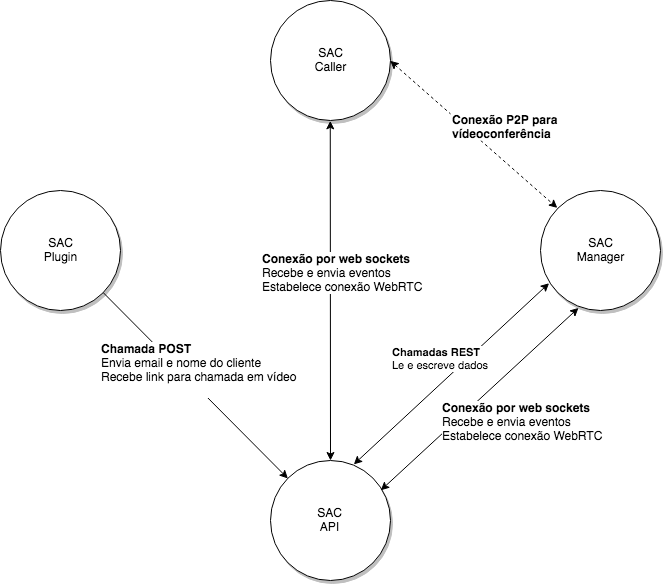
\includegraphics[scale=0.6]{figures/system-architecture.png} 
	\caption{Arquitetura dos projetos do sistema}
	\label{fig:system_architecture}
\end{figure}

Observamos na \autoref{fig:system_architecture} como os projetos estão organizados. O projeto \textit{SAC API} é um servidor com uma API REST que possui suporte a conexão \textit{web sockets} para a facilidade de troca de mensagens. Já SAC \textit{Manager}, \textit{Caller} e \textit{Plugin} são os três constituídos somente de HTML, Javascript e CSS, sendo os dois primeiros aplicações feitas em React.

Na figura \autoref{fig:webrtc_conn_flow} está explicado como é o fluxo para realizar uma conexão entre cliente e usuário:

\begin{figure}[ht!]
	\centering
    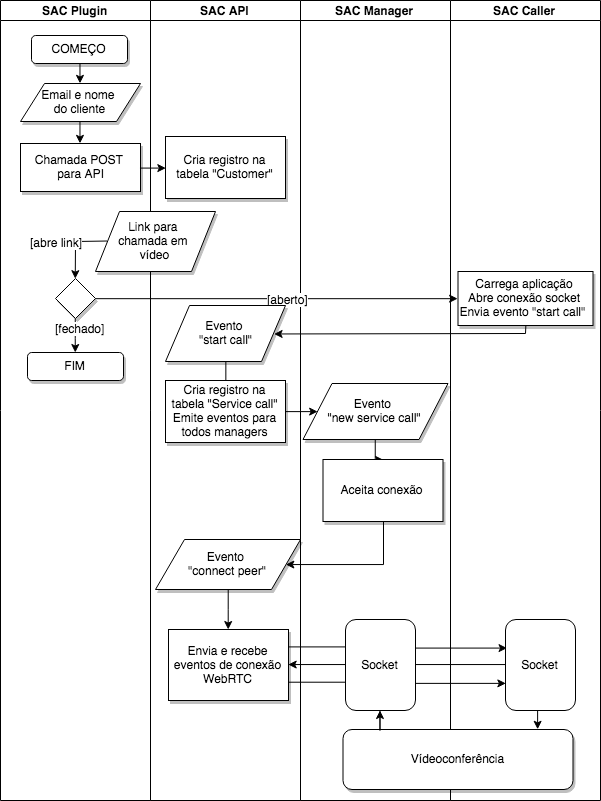
\includegraphics[scale=0.6]{figures/webrtc-conn-flow.png}
	\caption{Fluxograma conexão WebRTC entre cliente e usuário}
	\label{fig:webrtc_conn_flow}
\end{figure}

\clearpage
\subsection{Projeto SAC \textit{Manager}}

Aplicação feita com o propósito de ajudar os atendentes do sistema de atendimento a receberem chamadas de clientes, controlarem seus tickets, checarem se os problemas foram resolvidos entre outras funcionalidades.

No momento da inicialização é feita uma requisição ao servidor para coletar todos os dados do atendente junto das chamadas que ainda não foram atendidas, assim o mesmo pode responde-las mesmo não estando autenticado no momento da ligação.

O projeto é composto de quatro telas e a lista de chamadas:

\subsubsection{Login}

Tela de login básica (\autoref{fig:manager_login}) onde o atendente se autentica para receber as ligações que ele já realizou e para realizar outras e ter sua conta anexadas a ela. Não existe uma tela de cadastro pois o administrador do sistema deve fazer o cadastro de atendentes manualmente.

\begin{figure}[ht!]
	\centering
    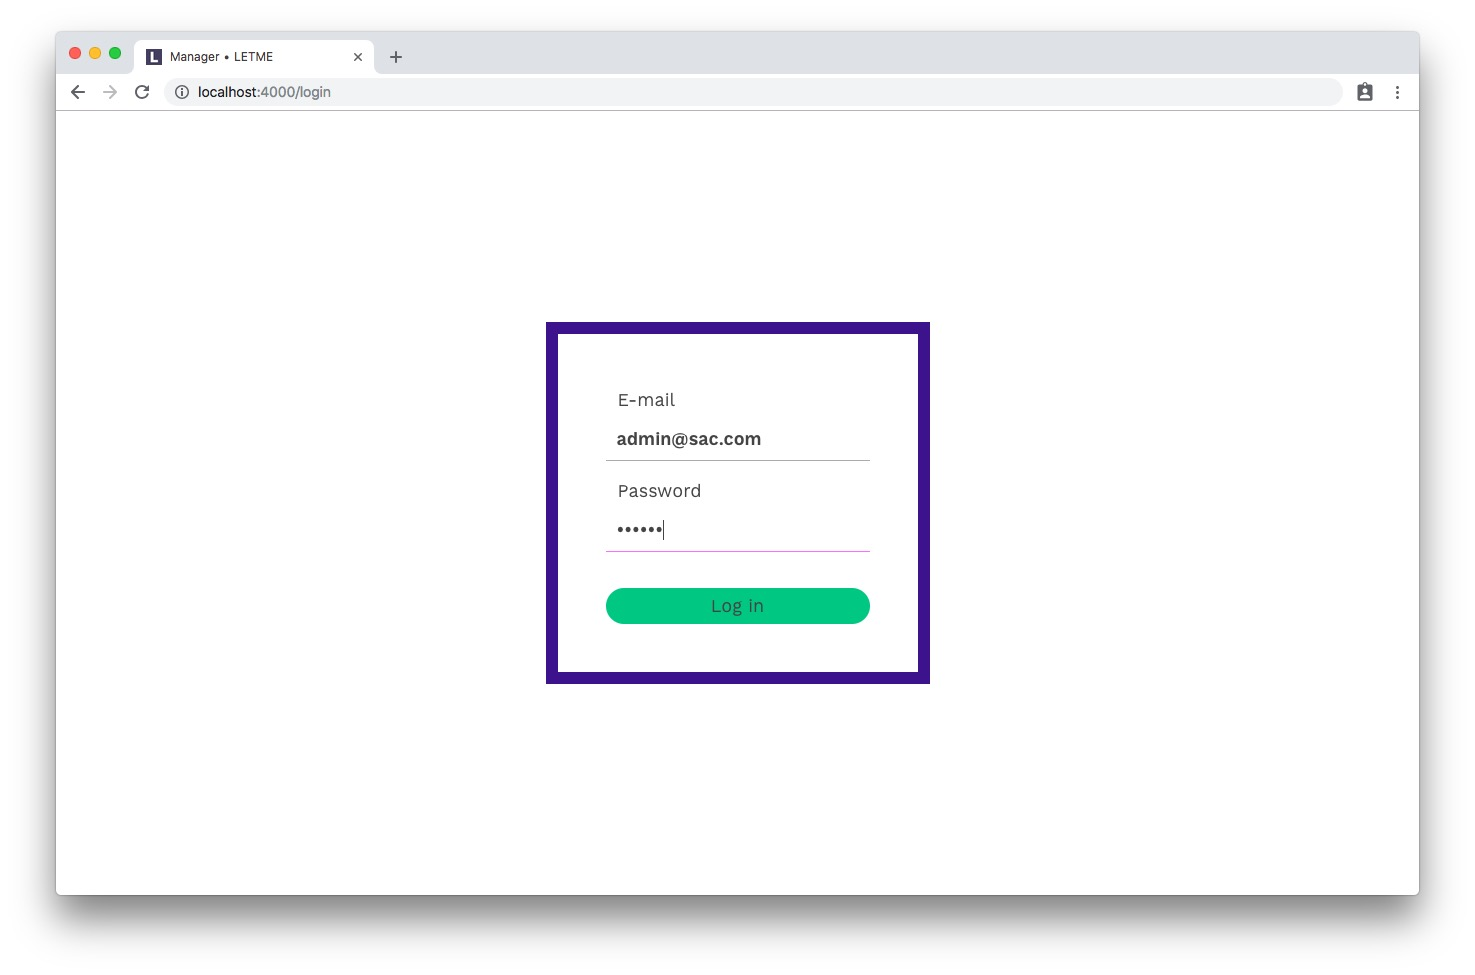
\includegraphics[scale=0.3]{figures/screens/manager-login.jpg}
	\caption{Tela de login do atendente}
	\label{fig:manager_login}
\end{figure}

\subsubsection{Vídeoconferência}

Principal tela do sistema onde o atendente consegue realizar o chamada de serviço e tentar resolver o problema do cliente. É nessa tela que a conexão \textit{peer-to-peer} é realizada. O vídeo é transmitido através de \textit{streams} disponibilizadas pela a API WebRTC do navegador.

Observamos na primeira tela (\autoref{fig:manager_video_overlay}) que o atendente está esperando a conexão com o cliente e o software oferece a possibilidade de desligar a ligação e como também ter uma visão da sua própria câmera.

\begin{figure}[ht!]
	\centering
    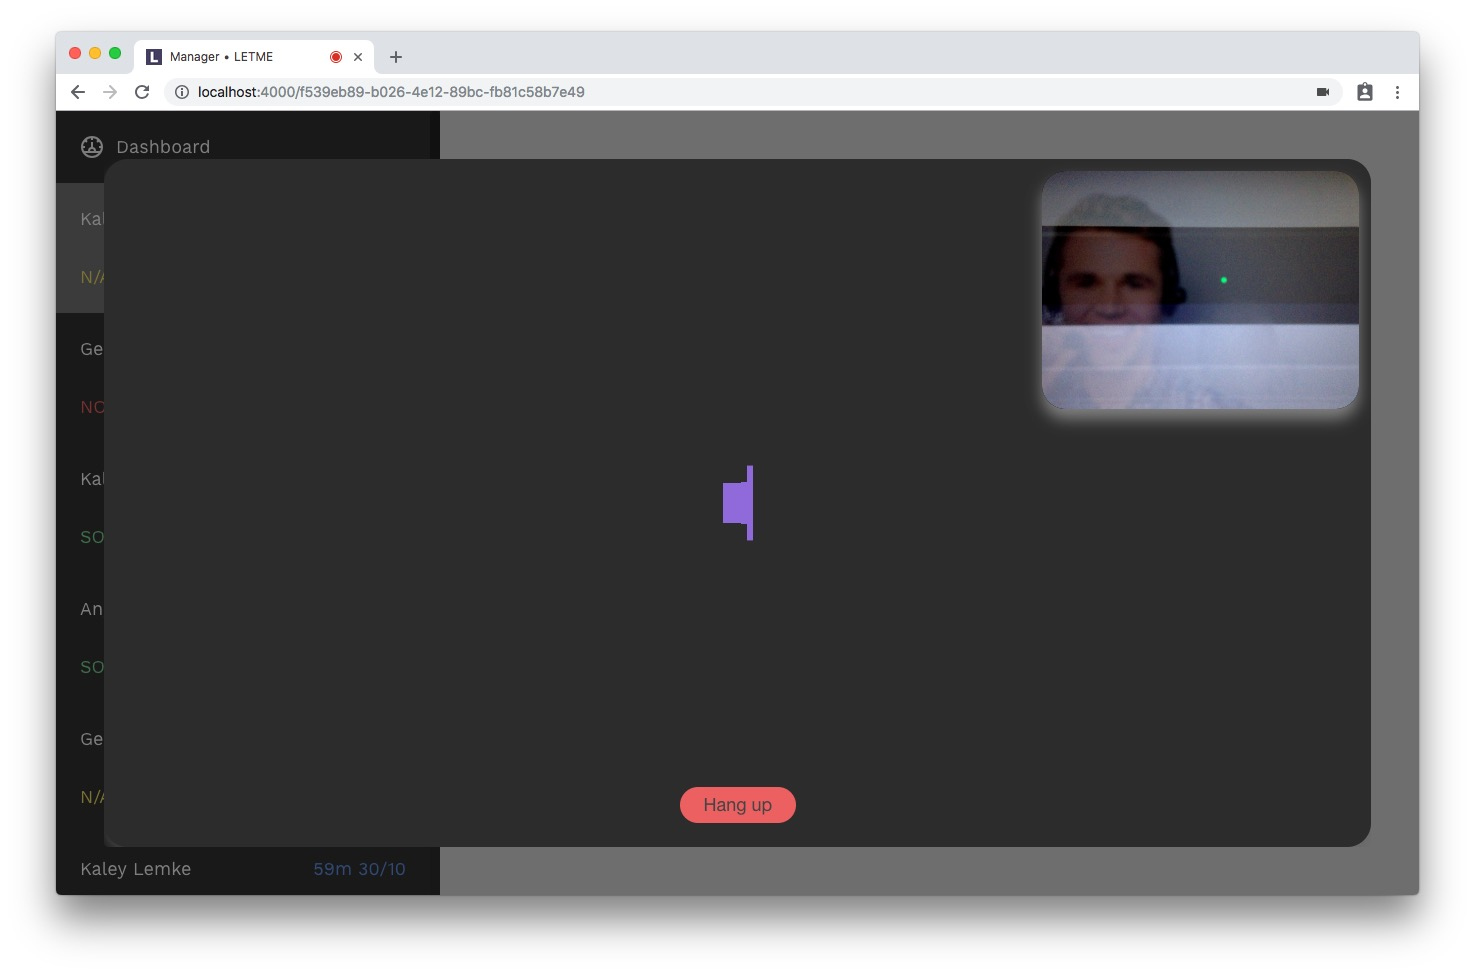
\includegraphics[scale=0.25]{figures/screens/manager-video-overlay.jpg}
	\caption{Atendente esperando conexão com cliente}
	\label{fig:manager_video_overlay}
\end{figure}

E na segunda tela (\autoref{fig:manager_video_chat}) vemos o cliente já conectado ao atendente.

\begin{figure}[ht!]
	\centering
    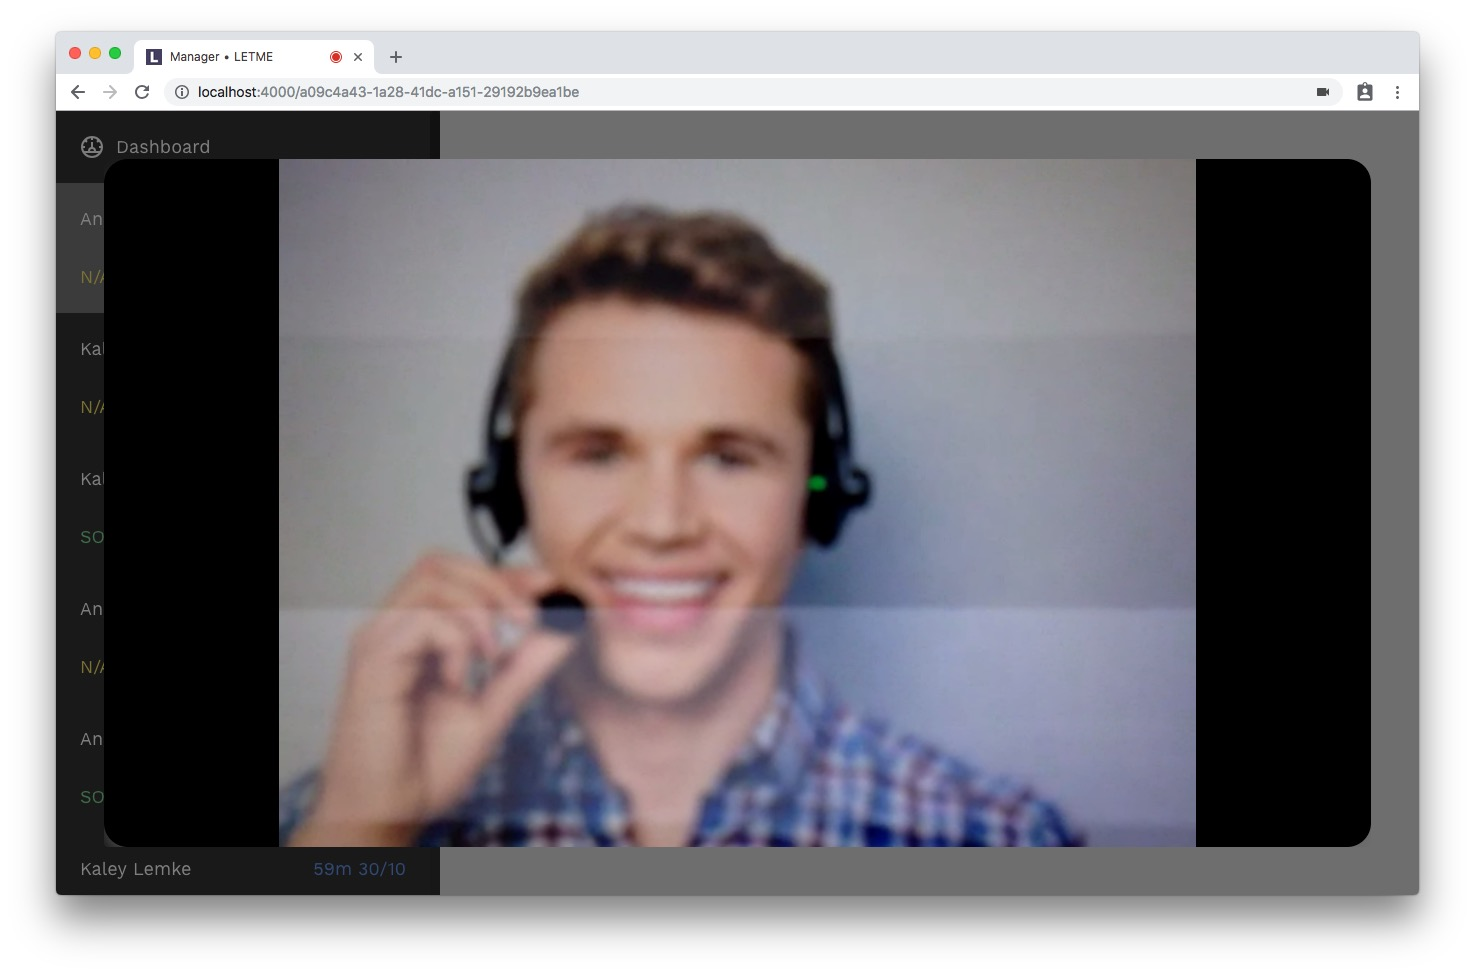
\includegraphics[scale=0.25]{figures/screens/manager-video-chat.jpg}
	\caption{Cliente aparecendo para o atendente}
	\label{fig:manager_video_chat}
\end{figure}

\subsubsection{Estatísticas do atendente}

Segunda tela mais importante, reúne informações de todas as ligações que o atendente fez, sintetizadas em um único lugar através de indicadores como média (\textit{avg}) e comparação entre ligações resolvidas e não resolvidas. 

\begin{figure}[ht!]
	\centering
    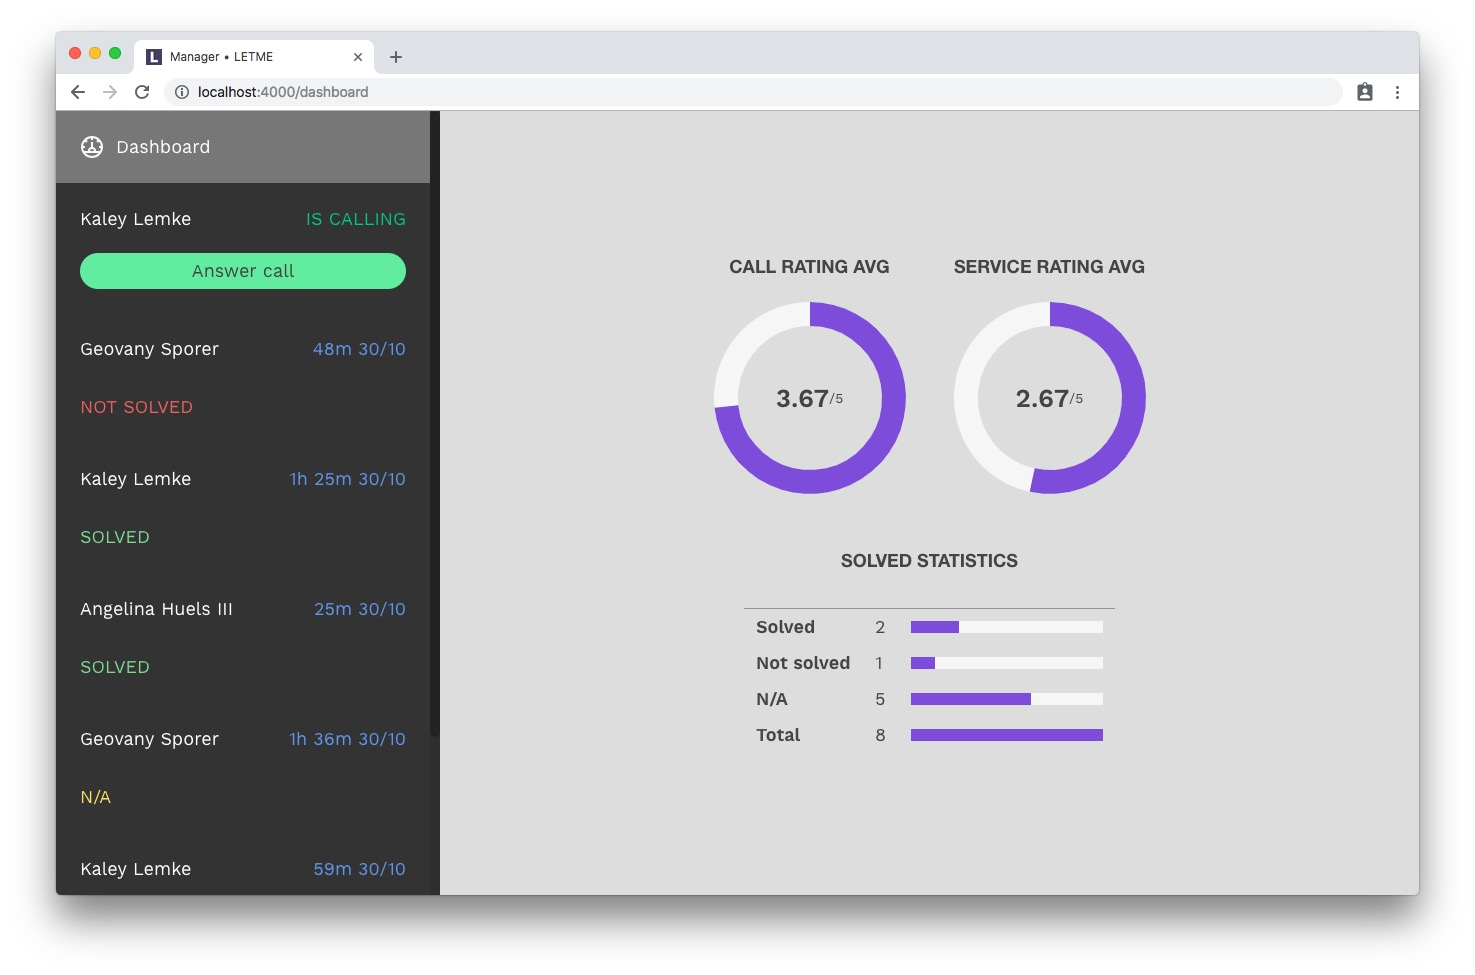
\includegraphics[scale=0.3]{figures/screens/manager-dashboard.jpg}
	\caption{Estatísticas do atendente}
	\label{fig:manager_dashboard}
\end{figure}


Vemos em \autoref{fig:manager_dashboard} que existem dados especificados como \textit{N/A} (sem resposta). Isso é devido ao usuário ter a possibilidade de fechar a janela do navegador sem ter respondido o questionário de \textit{feedback} no final da ligação.

\clearpage
\subsubsection{Estatísticas da ligação}

Tela utilizada para saber em mais detalhes informações sobre a chamada de serviço realizada. Nela temos outras informações como descrição da chamada que é fornecida pelo cliente e dados do mesmo, para que contatos futuros possam ser realizados se o problema não for resolvido.

\begin{figure}[ht!]
	\centering
    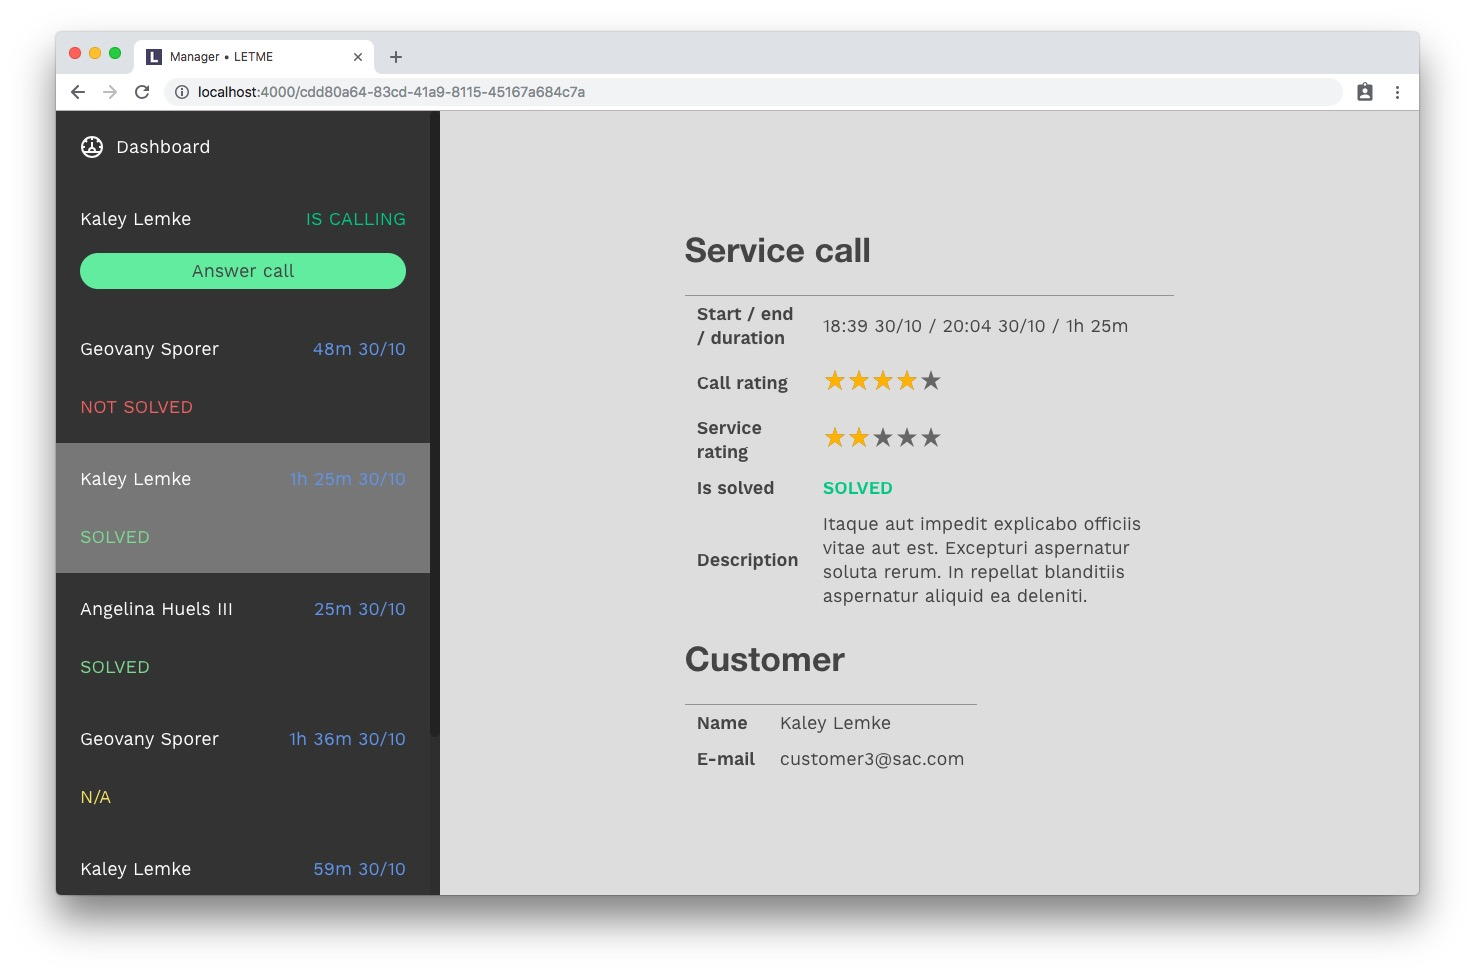
\includegraphics[scale=0.3]{figures/screens/manager-service-call.jpg}
	\caption{Estatísticas da ligação}
	\label{fig:manager_service_call}
\end{figure}

Observamos na imagem (\autoref{fig:manager_service_call}) avaliações da chamada (\textit{call}) e do serviço (\textit{service}). Como também informações de data e duração da mesma.

\clearpage
\subsubsection{Lista de chamadas}

Outra parte crucial do projeto, onde temos um visão rápida sobre as chamadas que foram realizadas e também sobre cliente que estão ligando no momento. 

\begin{figure}[ht!]
	\centering
    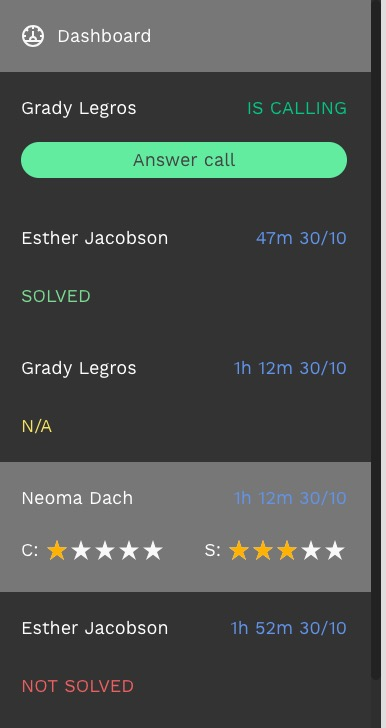
\includegraphics[scale=0.4]{figures/screens/manager-service-call-list.jpg}
	\caption{Lista de chamadas de serviço}
	\label{fig:manager_service_call_list}
\end{figure}

A lista (\autoref{fig:manager_service_call_list}) é atualizada em tempo real através de \textit{web sockets}, ou seja, não é necessário atualizar a página e fazer uma requisição ao servidor. Ao mesmo tempo quando uma chamada é atendida por outro usuário a mesma desaparece da lista. Cada atendente somente consegue visualizar suas próprias chamadas.

\clearpage
\subsection{Projeto SAC \textit{Caller}}

Projeto com o propósito de ser simples e pequeno para que não seja necessário o cliente baixar uma aplicação grande através de sua conexão 3G (caso Wi-Fi não esteja disponível). Essa parte do sistema conta com duas telas, a principal que realiza a conexão em vídeo e a outra, um formulário de qualidade para o cliente responder sobre a chamada.

O projeto funciona tanto em telas pequenas como grandes, porém como é muito parecido com o \textit{manager} a tela foi reduzida para demonstrar a sua capacidade.

\subsubsection{Vídeoconferência}

Tela mais importante do projeto onde o cliente faz a requisição de chamada para o sistema, e a requisição aparece na lista de chamadas (\autoref{fig:manager_service_call_list}) dos atendentes. O funcionamento é muito similar à videoconferência do \textit{manager}.

\begin{figure}[ht!]
	\centering
    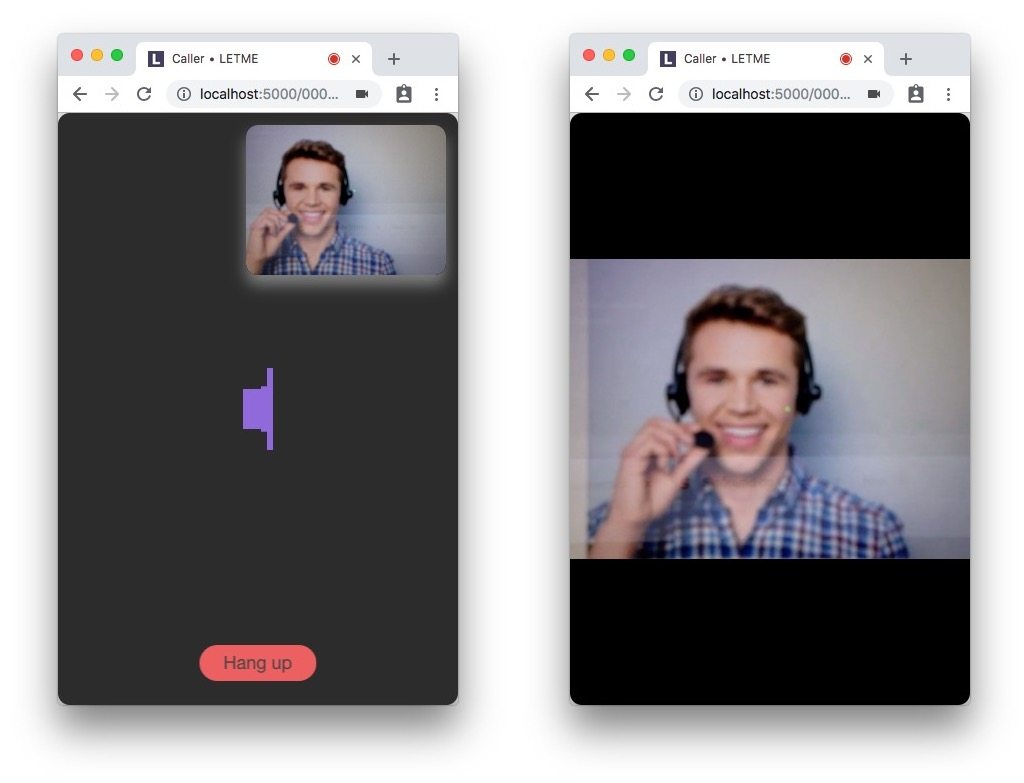
\includegraphics[scale=0.35]{figures/screens/caller-video-chat-overlay.jpg}
	\caption{Cliente em vídeoconferência}
	\label{fig:caller_video_chat_overlay}
\end{figure}

\subsubsection{Formulário de qualidade}

Vemos na figura (\autoref{fig:caller_feedback_form}) o formulário fornecido ao cliente após o fim da ligação.

\begin{figure}[ht!]
	\centering
    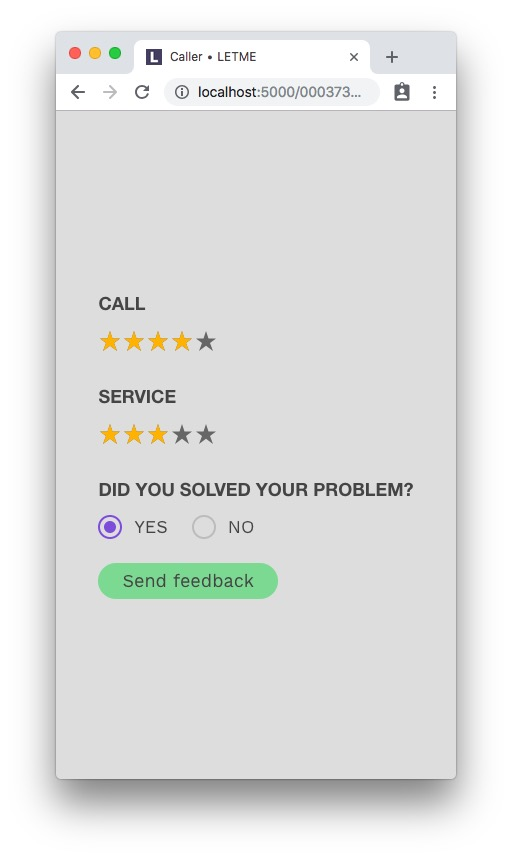
\includegraphics[scale=0.35]{figures/screens/caller-feedback-form.jpg}
	\caption{Formulário de qualidade fornecido ao cliente}
	\label{fig:caller_feedback_form}
\end{figure}

A funcionalidade do formulário tem como objetivo reunir informações tanto da qualidade do atendente como da qualidade da chamada em si (áudio, vídeo). E por fim se o problema do cliente foi resolvido ou não. Em futuras atualizações do software esse tipo de dado por ser utilizado para a empresa ter conhecimento sobre o próprio produto e sobre pontos de dor dos usuários.

